Die Entwicklung eines Softwaresystems ist ein wiederholendes Prozess, das sich in mehreren Phasen unterteilen lässt.
Alle Phasen beeinflüssen sich gegenseitig, sodass man sie nicht unabhängig voneinander betrachten kann. 

Die unterer Abbildung zeigt eine mögliche Aufteilung in Phasen der Entwicklung. 
\begin{figure}[H]
    \centering
    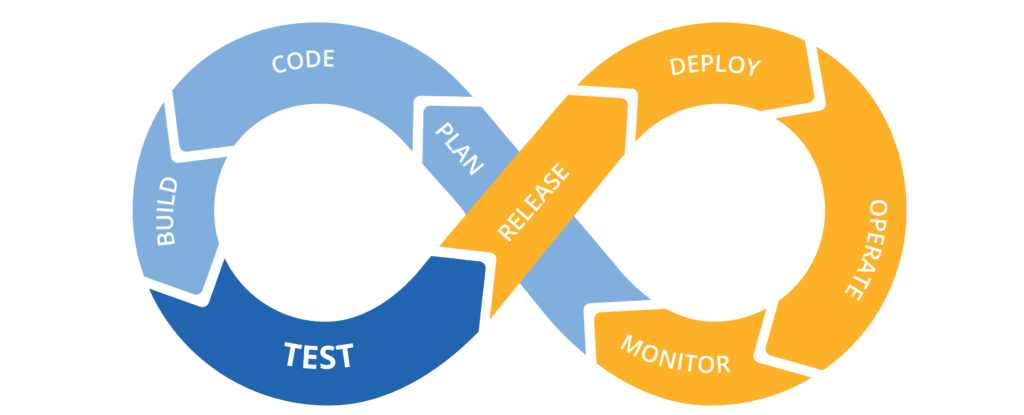
\includegraphics[width=1\textwidth]{../images/CiCD.png}
    \caption{CI/CD Pipeline}
    \label{fig:flow around cylinder}
    \source{https://blog.itil.org/2016/07/wort-zum-montag-cd-continous-delivery/}
\end{figure}

Man ist sehr daran interessiert, die Gesamtzeit des Zyklus so klein wie möglich zu halten, denn somit können die neuen Funktionalität schneller von Kunden benutzt werden und 
die Bugs werden schneller eliminiert. 

Im groben kann man die Entwicklung in 2 Teilen teilen: Bevor die neue Version der Software freigegeben wird und nach der Freigabe der neuen Version.
Die Phasen nach der Freigabe der neuen Version lassen sich fast vollständig automatisieren 
und verbrauchen dementsprechend nicht so viel Ressourcen ab einem gewissen Moment. Das großte Anteil an Ressourcen wird in die ersten 4 Phasen (Plan, Code, Build, Test) verbraucht, 
denn diese Aufgaben lassen sich sehr schlecht bis zu gar nicht automatisieren. 
Und wenn man am Anfang des Projektes schlechte Entscheidungen trifft, 
die das automatisierte Testen erschweren oder durch die schlechte Struktur des Programms das Hinzufügen der neuen Funktionalität deutlich schwieriger macht, 
wird man deutlich mehr Ressourcen gebrauchen, um das gleiche Ziel zu ereichen als wenn man das nicht gemacht hätte.

In dieser Arbeit wird es darum gehen, welche Entscheidungen am Beispiel eines OCPP Servers man bereits in der Phase ``Plan'' und ``Code'' treffen kann, 
um die Gesamtqualität der Software zu erhöhen, die die Anzahl an benötigten menschlichen Ressourcen reduziert. 